\section{Entwurf}
\subsection{Schichtenarchitektur}
Die Anwendung wird in drei Schichten unterteilt, in aufsteigender Reihenfolge sind
dies die Datenabstraktionsschicht, die Anwendungslogikschicht und die Darstellungsschicht. Die
hierbei erkennbare Nähe zum ``Model View Controller''-Entwurfsmuster\footnote{siehe
\url{https://de.wikipedia.org/wiki/Model_View_Controller}} ist beabsichtigt und
im Hinblick auf die (hypothetische) nächste Ausbaustufe dieser Software --
nämlich den Schritt hin zu einer verteilten Multi-User-Anwendung, z.B. durch eine
über das Netzwerk angebundene, gemeinsam genutzte Datenbank -- sogar unerlässlich.

Jede Schicht abstrahiert ihre jeweilige Kernaufgabe von der nächsthöheren Schicht.
Abhängigkeiten sind jeweils nur unidirektional zwischen einer Schicht und
den darunterliegenden Schichten bzw. externen Bibliotheken erlaubt.

Eine Schicht kann -- z.B. zu Testzwecken -- komplett ausgetauscht werden; die
Schnittstelle zwischen den Schichten wird fest durch deren jeweilige Header-Files
definiert und ist unabhängig von der konkreten Implementierung. Eine
Schichtimplementierung darf insbesondere nicht Funktionalität, die über die
Standardschnittstelle hinaus geht, höheren Schichten zur Verfügung.

\subsubsection{Datenabstraktionsschicht}
\label{datenabstraktionsschicht}
Die Datenabstraktionsschicht stellt die unterste Schicht der Anwendung dar.
Ihre Aufgabe ist die Umsetzung einer prinzipiell format- und speichermedienunabhängigen
CRUD\footnote{Create, Read/Query, Update, Delete}-Schittstelle, welche alle Datensätze
(und Operationen darauf) innerhalb einer Datenbank abbilden kann.

Hierzu gehören auch abstrakte Query-Operationen (prepared Statements), die im
einfachsten Fall schlicht an die zugrunde liegende SQL-Bibliothek weitergegeben
werden.

Operationen der Datenabstraktionsschicht schreiben / lesen direkt (bzw. unerheblich
gepuffert) in die Datenbank. Hierbei ist auf Nichtverletzung des ACID-Prinzips\footnote{Siehe
\url{https://de.wikipedia.org/wiki/ACID}} zu achten --- dies wird insbesondere durch die Benutzung
von Transaktionen und -- in der Standardimplementierung -- durch das Verwenden von SQLite als
zugrundeliegende Datenbank erreicht.

\subsubsection{Anwendungslogikschicht}
Die Anwendungslogikschicht stellt der Darstellungsschicht auf hoher Abstraktionsebene Such-, Abfrage-
und Sortierfunktionen sowie eine Transaktionsverwaltung mit Historie (für die
``Rückgängig''-Funktion) und einige Helferfunktionen, die von der Benutzeroberfläche
unabhängig sind (und bleiben sollen) zur Verfügung.

\subsubsection{Darstellungsschicht}
In der Darstellungsschicht werden schließlich Nutzereingaben entgegengenommen und
Datensätze wiedergegeben. Dies wird in diesem Fall wie gefordert über GTK+ umgesetzt,
kann aber theoretisch auch z.B. über ein via REST-API angebundenes HTML5-Frontend
realisiert werden.

Es ist möglich (und auch durchaus sinnvoll), die Anwendungslogikschicht als Bibliothek
aufzubauen und zu kompilieren, um dann verschiedenste Arten von Darstellungsschichten
nur noch gegen diese Bibliothek zu linken.

\subsection{Schnittstellenentwurf}
Da sich die objektorientierte Natur der UML nur schwer vollständig auf ein C-Programm
übertragen lässt, wird an dieser Stelle auf einen Schnittstellenentwurf und ein
UML-Klassendiagramm verzichtet. Es wird auf die entsprechenden Header-Files der
jeweiligen Module verwiesen, welche problemlos im Quellcodepaket auffindbar sind.

\subsection{Datenbankentwurf}
Die relationale Datenbank, welche als Dateiformat auserkoren wurde, ist äußerst
einfach aufgebaut:

\begin{center}
\noindent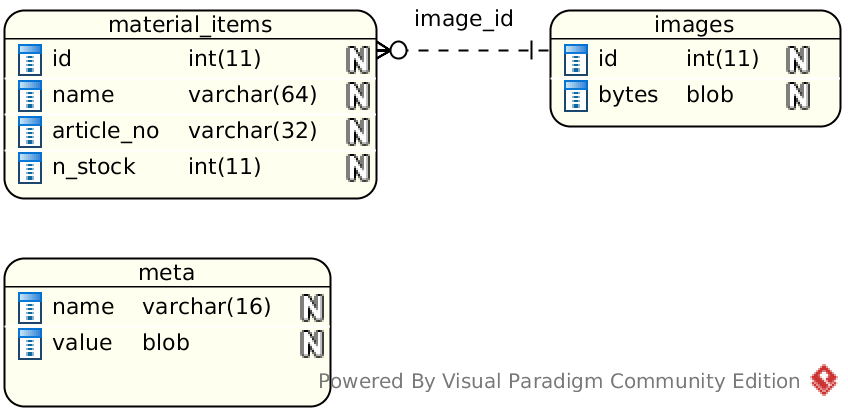
\includegraphics[width=110mm,keepaspectratio]{images/03-datenbankmodell.png}
\end{center}

Zusätzlich zum Domänenmodell ist hier lediglich die Tabelle ``meta'' neu: In ihr können
Konfigurations- und Metadaten aller Art gespeichert werden. Vorwiegend wird sie dafür
verwendet, die Version des Verwendeten Formats zu erfassen, sodass auch mit früheren
(oder späteren) Versionen der Anwendung erstellte Datenbanken verarbeitet werden können.

Der zum Aufbau dieser Datenbank erforderliche SQL-Code befindet sich bei den Quellcodes
zur Datenabstraktionsschicht.

\subsection{Anwendungsfälle und Screen Design}